% !Mode:: "TeX:UTF-8"
\chapter{后端2}
\begin{mdframed}  
	\textbf{主要目标}
	\begin{enumerate}[labelindent=0em,leftmargin=1.5em]
		\item 理解Sliding Window优化。
		\item 理解Pose Graph优化。
		\item 理解带IMU紧耦合的优化。
		\item 通过实验掌握g2o的Pose Graph与IMU紧耦合。
	\end{enumerate}
\end{mdframed}

上一讲我们重点介绍了以BA为主的图优化。BA能精确地优化每个相机位姿与特征点位置。不过在更大的场景中,大量特征点的存在会严重降低计算效率,导致计算量越来越大以至于无法实时化。本讲的第一部分要介绍一种简化的BA:位姿图。

当机器人上携带IMU传感器时,我们也可以通过IMU来计算图像帧间的相对运动。同样的,IMU的测量数据亦可作为优化观测量,放入图优化之中。本讲的第二部分将介绍VIO中的主流优化方法:IMU紧耦合。这需要读者熟练掌握先前介绍的图优化方法。

\newpage
\section{滑动窗口滤波和优化}
\subsection{实际环境下的BA结构}
带有相机位姿和空间点的图优化称为BA,能够有效地求解大规模的定位与建图问题。这在SfM问题中十分有用,但是在SLAM过程中,我们往往需要控制BA的规模,保持计算的实时性。倘若计算能力无限,那不妨每时每刻都计算整个BA好了——但是那不符合现实。现实条件是,我们必须限制后端的计算时间,比如迭代不超过20次,用时不超过0.5秒,等等。像SfM那样用一周时间去重建一个城市地图的算法,在SLAM里不见得有效。

控制计算规模的做法有很多,比如从连续的视频中抽出一部分作为\textbf{关键帧}\textsuperscript{\cite{Leutenegger2015}},仅构造关键帧与路标点之间的BA,于是非关键帧只用于定位,对建图则没有贡献。即便如此,随着时间的流逝,关键帧数量会越来越多,地图规模也将不断增长。像BA这样的批量优化方法,计算效率会(令人担忧地)不断下降。为了避免这种情况,我们需要用一定手段来控制后端BA的规模。这些手段可以是理论上的,也可以是工程上的。

例如,最简单的控制BA规模的思路,是仅保留离当前时刻最近的$N$个关键帧,去掉时间上更早的关键帧。于是,我们的BA将被固定在一个时间窗口内,离开这个窗口的则被丢弃。这种方法称为滑动窗口(Sliding Window)法\textsuperscript{\cite{Sibley2008}}。当然,取这$N$个关键帧的具体方法可以有一些改变,比方说,不见得必须取时间上最近的,而可以按照某种原则,取时间上靠近,空间上又可以展开的关键帧,从而保证相机即使在停止不动时,BA的结构不至于缩成一团(这容易导致一些糟糕的退化情况)。如果我们在帧与帧的结构上再考虑的深一些,也可以像ORB-SLAM2\textsuperscript{\cite{Mur-Artal2015}}那样,定义一种称为“共视图”(Covisibility graph)的结构(见\autoref{fig:cov-graph})。所谓共视图,就是指那些“与现在的相机存在共同观测的关键帧构成的图)。于是,在BA优化时,我们按照某些原则在共视图内取一些关键帧和路标进行优化,比方说与当前帧有20个以上共视路标的关键帧,对其他的保持不变。当共视图关系能够正确构造的时候,基于共视图的优化也会在更长时间内保持最优。

\begin{figure}[!ht]
	\centering
	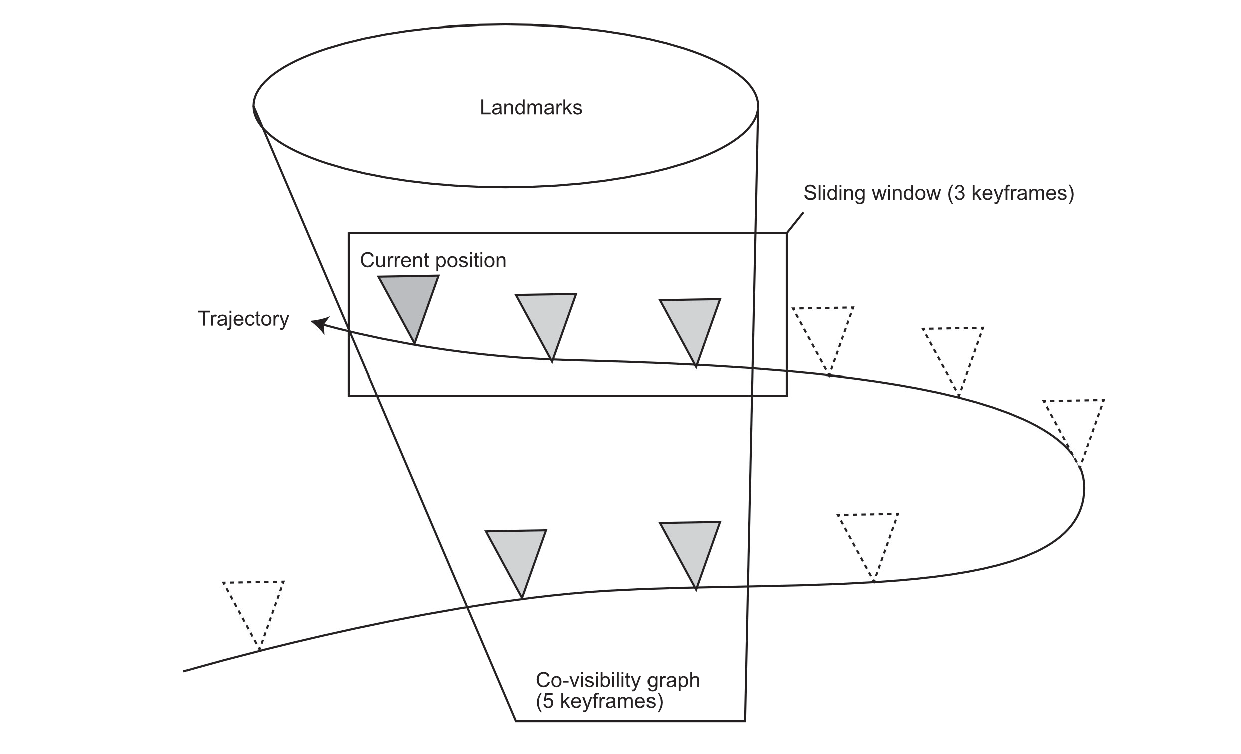
\includegraphics[width=0.8\textwidth]{backend2/cov-graph.pdf}
	\caption{滑动窗口和共视图的示意图}
	\label{fig:cov-graph}
\end{figure}

滑动窗口也好,共视图也好,大体而言,都是我们对实时计算的某种工程上的折中。不过在理论上,它们也引入了一个新问题:刚才我们谈到要“丢弃”滑动窗口之外,或者“固定”共视图之外的变量,这个“丢弃”和“固定”具体是怎样一个操作?“固定”似乎很容易理解,我们只需将共视图之外的关键帧估计值保持不变即可。但是“丢弃”,是指完全弃置不用,即窗口外的变量完全不对窗口内的变量产生任何影响,还是说窗口外的数据\textbf{应该}有一些影响,但实际上被我们忽略了?如果有影响,这种影响应该是什么样子?它够不够明显,能不能忽略?

接下来我们就要谈谈这些问题。它们在理论上应该如何处理,以及在工程上能不能做一些简化手段。

\subsection{滑动窗口法}
现在考虑一个滑动窗口。假设这个窗口内有$N$个关键帧,它们的位姿表达为:$$\bm{x}_1, \ldots, \bm{x}_N,$$我们假设它们在向量空间,即用李代数表达,那么,关于这几个关键帧,我们能谈论些什么呢?

显然我们关心这几个关键帧的位置在哪里,以及它们的不确定度如何,这对应着它们在高斯分布假设下的均值协方差。如果这几个关键帧还对应着一个局部地图,我们也可以顺带着问整个局部系统的均值和方差应该是多少。设这个滑动窗口中还有$M$个路标点:$\bm{y}_1, \ldots, \bm{y}_N$,它们与$N$个关键帧组成了局部地图。显然我们可以用上一讲节介绍的Bundle Adjustment方法处理这个滑动窗口,包括建立图优化模型,构建整体的Hessian矩阵,然后边缘化所有路标点来加速求解。在边缘化时,我们考虑关键帧的位姿,即$$[\bm{x}_1, \ldots, \bm{x}_N]^\mathrm{T} \sim N([\boldsymbol{\mu}_1, \ldots, \boldsymbol{\mu}_N]^\mathrm{T},  \boldsymbol{\Sigma}).$$ 其中$\boldsymbol{\mu}_k$为第$k$个关键帧的位姿均值,$\boldsymbol{\Sigma}$为所有关键帧的协方差矩阵,那么显然,均值部分就是指BA迭代之后的结果,而$\boldsymbol{\Sigma}$就是对整个BA的$\bm{H}$矩阵进行边缘化之后的结果,即上一讲提到的矩阵$\bm{S}$。我们认为读者已经熟悉这个流程了。

在滑动窗口中,我们另一个问题是问,当窗口结构发生改变,这些状态变量应该如何变化?这件事情可以分成两部分讨论:
\begin{enumerate}
\item 我们需要在窗口中新增一个关键帧,以及它观测到的路标点。
\item 我们需要把窗口中一个旧的关键帧删除,同时也可能删除它观测到的路标点。	
\end{enumerate}

这时,滑动窗口法和传统的BA的区别就显现出来。显然,如果按照传统的BA来处理,那么这仅仅对应于两个不同结构的BA,在求解上没有任何差别。但如果在滑动窗口的情况下,我们就要讨论这些具体的细节问题了。

\subsubsection{新增一个关键帧和路标点}
考虑在上个时刻,滑动窗口已经建立了$N$个关键帧,我们也已知道它们服从某个高斯分布,其均值和方差如前所述。此时,新来了一个关键帧$\bm{x}_{N+1}$,那么整个问题中的变量变为$N+1$个关键帧和更多路标点的集合。这实际上仍是平凡的,我们只需按照正常的BA流程处理即可。对所有点进行边缘化时,即得到这$N+1$个关键帧的高斯分布参数。

\subsubsection{删除一个旧的关键帧}
当考虑删除旧关键帧时,一个理论问题将显现出来。比方说我们要删除旧关键帧$\bm{x}_1$,但是$\bm{x}_1$并不是孤立的,它会和其他帧观测到同样的路标。将$\bm{x}_1$边缘化之后将导致整个问题不再稀疏。和上一讲一样,我们举一个示意图,如\autoref{fig:marg-frame}所示。

\begin{figure}[!ht]
    \centering
    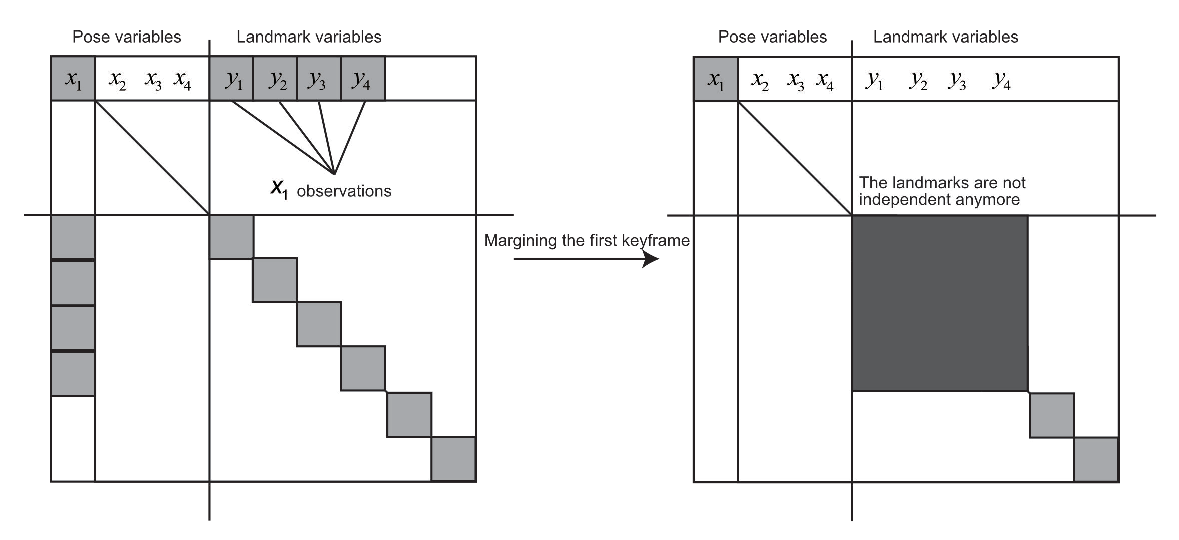
\includegraphics[width=0.8\textwidth]{backend2/marg-frame.pdf}
    \caption{滑动窗口删除关键帧将破坏路标部分的对角块结构}
    \label{fig:marg-frame}
\end{figure}

在这个例子中,我们假设$\bm{x}_1$看到了路标点$\bm{y}_1$至$\bm{y}_4$,于是,在处理之前,BA问题的Hessian矩阵应该像这个图的左侧一样,在$\bm{x}_1$行的$\bm{y}_1$到$\bm{y}_4$列存在着非零块,表示$\bm{x}_1$看到了它们。这时考虑边缘化$\bm{x}_1$,那么Schur消元过程相当于通过矩阵行和列操作消去非对角线处几个非零矩阵块,显然这将导致右下角的路标点矩阵块不再是非对角矩阵。这个过程称为边缘化中的\textbf{填入}(Fill-in)\textsuperscript{\cite{Sibley2008}}。

回顾上一讲的边缘化,当我们边缘点路标点时,Fill-in将出现在左上角的位姿块中。不过,因为BA不要求位姿块为对角块,所以稀疏BA求解仍然可行。但是,当边缘化关键帧时,将破坏右下角路标点之间的对角块结构,这时BA就无法按照先前的稀疏方式迭代求解。这显然是个十分糟糕的问题。实际上,在早期的EKF滤波器后端中,人们确实保持着一个稠密的Hessian矩阵,这也使得EKF后端没法处理较大规模的滑动窗口。

不过,如果我们对边缘化的过程进行一些改造,也可以保持滑动窗口BA的稀疏性。比方说,在边缘化某个旧的关键帧时,同时边缘化它观测到的路标点。这样,路标点的信息就会转换成剩下那些关键帧之间的共视信息,从而保持右下角部分的对角块结构。在某些SLAM框架\textsuperscript{\cite{Leutenegger2015,Engel2016}}中,边缘化策略还会更复杂一些。例如在OKVIS中,我们会判断要边缘化的那个关键帧,它看到的路标点是否在最新的关键帧中仍能看到。如果不能,就直接边缘化这个路标点;如果能,那就丢弃被边缘化关键帧对这个路标点的观测,从而保持BA的稀疏性。

\subsubsection{SWF中边缘化的直观解释}
我们知道边缘化在概率上的意义就是指条件概率。所以直观来说,当我们边缘化某个关键帧,即是说,“保持这个关键帧当前的估计值,求其他状态变量以这个关键帧为条件的条件概率”。所以,当某个关键帧被边缘化,它观测到的路标点就会产生一个“\textbf{这些路标应该在哪里}”的先验信息,从而影响其余部分的估计值。如果再边缘化这些路标点,那么它们的观测者将得到一个“\textbf{观测它们的关键帧应该在哪里}”的先验信息。

从数学上看,当我们边缘化某个关键帧, 整个窗口中的状态变量的描述方式,将从联合分布变成一个条件概率分布。以上面的例子来看,就是说:
\begin{equation}
p\left( {{\bm{x}_1}, \ldots {\bm{x}_4},{\bm{y}_1}, \ldots {\bm{y}_6}} \right) = p\left( {{\bm{x}_2}, \ldots ,{\bm{x}_4},{\bm{y}_1}, \ldots {\bm{y}_6}|{\bm{x}_1}} \right)\underbrace {p\left( {{\bm{x}_1}} \right)}_{\text{舍去}}.
\end{equation}
然后舍去被边缘化部分的信息。在变量被边缘化之后,我们在工程当中就不应再使用它。所以滑动窗口法比较适合VO系统,而不适合大规模建图的系统。

由于现在g2o和Ceres还未直接支持滑动窗口法中的边缘化操作\footnote{工程当中我们可以通过某些巧妙的手段绕过g2o和Ceres的框架限制,但这往往非常繁琐,不适合在书中演示。},我们略去本节对应的实验部分。希望理论部分可以帮助读者理解一些基于滑动窗口的SLAM系统。

\section{位姿图(Pose Graph)}
\subsection{Pose Graph的意义}
根据前面的讨论,我们发现特征点在优化问题中占据了绝大部分。而实际上,经过若干次观测之后,那些收敛的特征点,空间位置估计会收敛至一个值保持不动,而发散的外点则通常看不到了。对收敛点再进行优化,似乎是有些费力不讨好的。因此,我们更倾向于在优化几次之后就把特征点固定住,只把它们看作位姿估计的约束,而不再实际地优化它们的位置估计。

沿着这个思路往下走,我们会想到:是否能够完全不管路标而只管轨迹呢?我们完全可以构建一个只有轨迹的图优化,而位姿节点之间的边,可以由两个关键帧之间通过特征匹配之后得到的运动估计来给定初始值。不同的是,一旦初始估计完成,我们就不再优化那些路标点的位置,而只关心所有的相机位姿之间的联系了。通过这种方式,我们省去了大量的特征点优化的计算,只保留了关键帧的轨迹,从而构建了所谓的位姿图(Pose Graph),如\autoref{fig:pose-graph}~所示。

\begin{figure}[!ht]
	\centering
	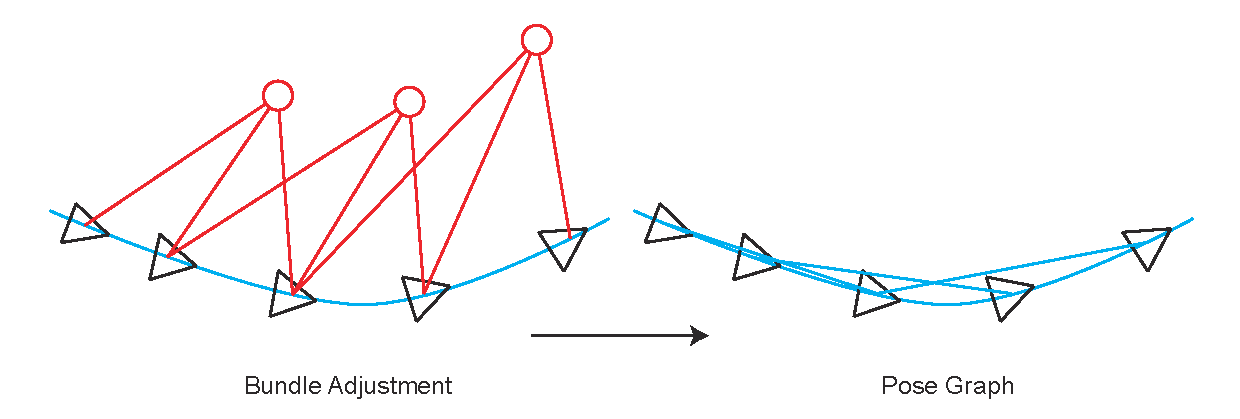
\includegraphics[width=0.8\textwidth]{backend2/posegraph.pdf}
	\caption{Pose Graph示意图。当我们不再优化Bundle Adjustment中的路标点,仅把它们看成对姿态节点的约束时,就得到了一个计算规模减小很多的Pose Graph。}
	\label{fig:pose-graph}
\end{figure}

我们知道,在BA中特征点数量远大于位姿节点。一个关键帧往往关联了数百个关键点,而实时BA的最大计算规模,即使利用稀疏性,在当前的主流CPU上一般也就是几万个点左右。这就限制了SLAM应用场景。所以,当机器人在更大范围的时间和空间中运动时,必须考虑一些解决方式:要么像滑动窗口法那样,丢弃一些历史数据\textsuperscript{\cite{Strasdat2011}};要么像Pose Graph的做法那样,舍弃对路标点的优化,只保留Pose之间的边,使用Pose Graph\textsuperscript{\cite{Dubbelman2015, Lee2014, Latif2013}}。此外,如果我们有额外测量Pose的传感器,那么Pose Graph也是一种常见的融合Pose测量的方法。


\subsection{Pose Graph的优化}
那么,Pose Graph图优化中的节点和边都是什么意思呢?这里的节点表示相机位姿,以$\bm{T}_1, \cdots, \bm{T}_n$来表达。而边,则是两个位姿节点之间相对运动的估计,该估计可能来自于特征点法或直接法,也可以来自GPS或IMU积分,但不管如何,我们估计了,比如说$\bm{T}_i$和$\bm{T}_j$之间的一个运动$\Delta \bm{T}_{ij}$。该运动可以有若干种表达方式,我们取比较自然的一种:
\begin{equation}
\Delta \bm{\xi}_{ij} = \bm{\xi}_i^{-1} \circ \bm{\xi}_j = \ln \left( \bm{T}_i^{-1} \bm{T}_j \right)^\vee,
\end{equation}
或按李群的写法:
\begin{equation}
\bm{T}_{ij} =\bm{T}_i^{-1} \bm{T}_j.
\end{equation}

按照图优化的思路,实际当中该等式不会精确地成立,因此我们设立最小二乘误差,然后和以往一样,讨论误差关于优化变量的导数。这里,我们把上式的$\bm{T}_{ij}$移至等式右侧,构建误差$\bm{e}_{ij}$:
\begin{equation}
\bm{e}_{ij} = \Delta \bm{\xi}_{ij} \ln \left( \bm{T}_{ij}^{-1} \bm{T}_i^{-1} \bm{T}_j \right)^\vee
\end{equation}

注意优化变量有两个:$\bm{\xi}_i$和$\bm{\xi}_j$,因此我们求$\bm{e}_{ij}$关于这两个变量的导数。按照李代数的求导方式,给$\bm{\xi}_i$和$\bm{\xi}_j$各一个左扰动:$ \bm{\delta \xi}_i$和$ \bm{\delta \xi}_j$。于是误差变为
\begin{equation}
\hat{ \bm{e}}_{ij} = \ln \left( \bm{T}_{ij}^{-1}  \bm{T}_i^{-1} \exp((-\bm{\delta \xi}_i)^\wedge) \exp(\delta \bm{\xi}_j^\wedge) \bm{T}_j  \right)^\vee.
\end{equation}

该式中,两个扰动项被夹在了中间。为了利用BCH近似,我们希望把扰动项移至式子左侧或右侧。回忆第4讲习题中的伴随性质,即式\eqref{eq:adjSE3}。如果你没有做过这个习题,那就暂时把它当作是正确的结论来使用:
\begin{equation}
\exp \left( \left( \mathrm{Ad}(\bm{T}) \bm{\xi} \right) ^\wedge \right) = \bm{T} \exp(\bm{\xi}^\wedge)\bm{T}^{-1}.
\end{equation}

稍加改变,有:
\begin{equation}
\exp(\bm{\xi}^\wedge)\bm{T} = \bm{T} \exp \left( \left( \mathrm{Ad}(\bm{T}^{-1}) \bm{\xi} \right) ^\wedge \right) .
\end{equation}

该式表明,通过引入一个伴随项,我们能够“交换”扰动项左右侧的$\bm{T}$。利用它,可以将扰动挪到最右(当然最左亦可),导出右乘形式的雅可比矩阵(挪到左边时形成左乘):
\begin{equation}
\begin{aligned}
\hat{ \bm{e}}_{ij} &= \ln \left( \bm{T}_{ij}^{-1}  \bm{T}_i^{-1} \exp((-\bm{\delta \xi}_i)^\wedge) \exp(\delta \bm{\xi}_j^\wedge) \bm{T}_j  \right)^\vee\\
&= \ln \left( \bm{T}_{ij}^{-1} \bm{T}_i^{-1} \bm{T}_j \exp \left( \left(- \mathrm{Ad}(\bm{T}_j^{-1}) \bm{\delta \xi}_i \right)^\wedge \right) \exp \left( \left( \mathrm{Ad}(\bm{T}_j^{-1})  \bm{\delta\xi}_j\right)^\wedge \right) \right)^\vee \\ 
&\approx \ln \left( \bm{T}_{ij}^{-1} \bm{T}_i^{-1} \bm{T}_j \left[ \bm{I} - (\mathrm{Ad}(\bm{T}_j^{-1}) \bm{\delta \xi}_i)^\wedge + (\mathrm{Ad}(\bm{T}_j^{-1})  \bm{\delta \xi}_j)^{\wedge} \right] \right)^\vee \\
& \approx \bm{e}_{ij} + \frac{\partial \bm{e}_{ij}}{\partial \bm{\delta \xi}_i} \bm{\delta \xi}_i + \frac{\partial \bm{e}_{ij}}{\partial \bm{\delta \xi}_j} \bm{\delta \xi}_j
\end{aligned}.
\end{equation}

因此,按照李代数上的求导法则,我们求出了误差关于两个位姿的雅可比矩阵。关于$\bm{T}_i$的:
\begin{equation}
\frac{\partial \bm{e}_{ij}}{\partial \bm{\delta \xi}_i} = - \bm{\mathcal{J}}_r^{-1}(\bm{e}_{ij}) \mathrm{Ad}(\bm{T}_j^{-1}).
\end{equation}
以及关于$\bm{T}_j$的:
\begin{equation}
\frac{\partial \bm{e}_{ij}}{\partial \bm{\delta \xi}_j} = \bm{\mathcal{J}}_r^{-1}(\bm{e}_{ij}) \mathrm{Ad}(\bm{T}_j^{-1}).
\end{equation}

如果读者觉得这部分求导理解起来有困难,可以回到第4讲温习一下李代数部分的内容。不过,前面也说过,由于$\mathfrak{se}(3)$上的左右雅可比$\bm{\mathcal{J}}_r$形式过于复杂,我们通常取它们的近似。如果误差接近于零,我们就可以设它们近似为$\bm{I}$或
\begin{equation}
\bm{\mathcal{J}}_r^{-1}(\bm{e}_{ij}) \approx \bm{I} + \frac{1}{2} 
\left[ 
{\begin{array}{*{20}{c}}
	{{\bm{\phi}_{\bm{e}} ^ \wedge }}&{{\bm{\rho}_{\bm{e}} ^ \wedge }}\\
	{\bm{0}}&{{\bm{\phi}_{\bm{e}} ^ \wedge }}
\end{array}} 
\right].
\end{equation}

理论上讲,即使在优化之后,由于每条边给定的观测数据并不一致,误差通常也不见得近似于零,所以简单地把这里的$\bm{\mathcal{J}}_r$设置为$\bm{I}$会有一定的损失。稍后我们将通过实践来看看理论上的区别是否明显。

了解雅可比求导后,剩下的部分就和普通的图优化一样了。简而言之,所有的位姿顶点和位姿——位姿边构成了一个图优化,本质上是一个最小二乘问题,优化变量为各个顶点的位姿,边来自于位姿观测约束。记$\mathcal{E}$为所有边的集合,那么总体目标函数为
\begin{equation}
\mathop {\min }\limits \frac{1}{2}\sum\limits_{i,j \in \mathcal{E}} \bm{e}_{ij}^\mathrm{T} \bm{\Sigma}_{ij}^{-1} \bm{e}_{ij}.
\end{equation}

我们依然可以用高斯牛顿法、列文伯格—马夸尔特方法等求解此问题,除了用李代数表示优化位姿以外,别的都是相似的。根据先前的经验,这自然可以用Ceres或g2o进行求解。我们不再讨论优化的详细过程,上一讲已经讲得够多了。

\section{实践:位姿图优化}
\subsection{g2o原生位姿图}
下面演示使用g2o进行位姿图优化。首先,请读者用g2o\_viewer打开我们预先生成的仿真位姿图,位于slambook2/ch10/sphere.g2o中,如\autoref{fig:sphere-before}~所示。

\begin{figure}[!htp]
	\centering
	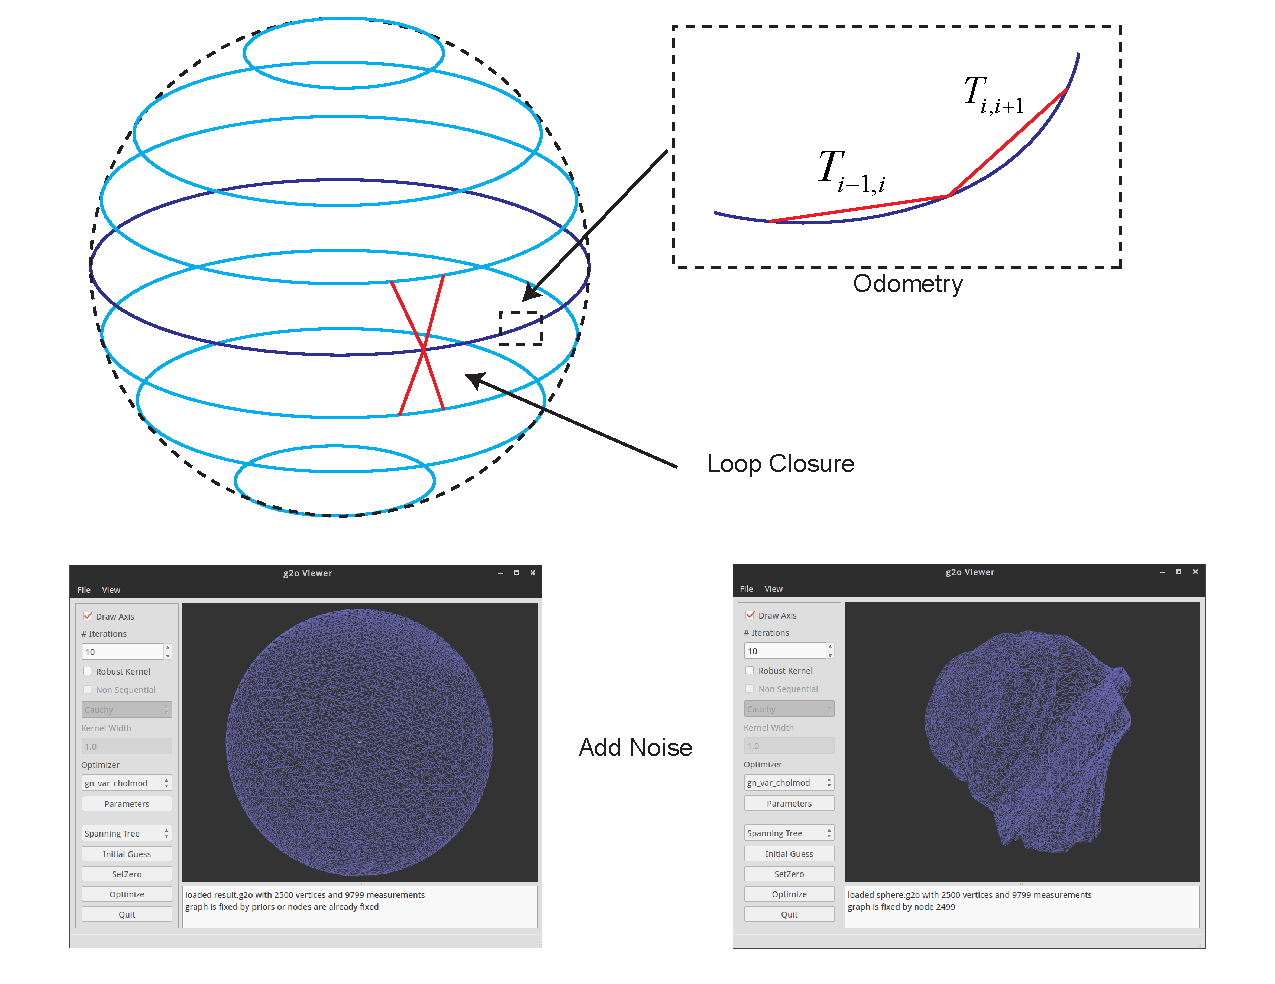
\includegraphics[width=1.0\textwidth]{backend2/sphere-before.pdf}
	\caption{g2o仿真产生的位姿图。真值是完整的球形,在真值上添加噪声后得到带累计误差的仿真数据。}
	\label{fig:sphere-before}
\end{figure}

该位姿图是由g2o自带的create sphere程序仿真生成的。它的真实轨迹为一个球,由从下往上的多个层组成。每层为一个正圆形,很多个大小不一的圆形层组成了一个完整的球体,共包含2500个位姿节点(\autoref{fig:sphere-before}~左上),可以看成一个转圈上升的过程。然后,仿真程序生成了$t-1$到$t$时刻的边,称为odometry边(里程计)。此外,又生成层与层之间的边,称为loop closure(回环,回环检测算法将在下一讲详细介绍)。随后,在每条边上添加观测噪声,并根据里程计边的噪声,重新设置节点的初始值。这样,就得到了带累积误差的位姿图数据(\autoref{fig:sphere-before}~右下)。它局部看起来像球体的一部分,但整体形状与球体相差甚远。现在我们从这些带噪声的边和节点初始值出发,尝试优化整个位姿图,得到近似真值的数据。

当然,实际当中的机器人肯定不会出现这样正球形的运动轨迹,以及如此完整的里程计与回环观测数据。仿真成正球的好处是我们能够直观地看到优化结果是否正确(只要看它各个角度圆不圆就行了)。读者可以单击g2o\_viewer中的optimize函数,看到每步的优化结果和收敛的过程。另一方面,sphere.g2o也是一个文本文件,可以用文本编辑器打开,查看它里面的内容。文件前半部分由节点组成,后半部分则是边:

\begin{lstlisting}
VERTEX_SE3:QUAT 0 -0.125664 -1.53894e-17 99.9999 0.706662 4.32706e-17 0.707551 -4.3325e-17 
......
EDGE_SE3:QUAT 1524 1574 -0.210399 -0.0101193 -6.28806 -0.00122939 0.0375067 -2.85291e-05 0.999296 10000 0 0 0 0 0 10000 0 0 0 0 10000 0 0 0 40000 0 0 40000 0 40000 
\end{lstlisting}

可以看到,节点类型是VERTEX\_SE3,表达一个相机位姿。g2o默认使用四元数和平移向量表达位姿,所以后面的字段意义为:ID,$t_x, t_y, t_z, q_x, q_y, q_z, q_w$。前3个为平移向量元素,后4个为表示旋转的单位四元数。同样,边的信息为两个节点的ID,$t_x, t_y, t_z, q_x, q_y, q_z, q_w$,信息矩阵的右上角(由于信息矩阵为对称阵,只需保存一半即可)。可以看到这里把信息矩阵设成了对角阵。

为了优化该位姿图,我们可以使用g2o默认的顶点和边,它们是由四元数表示的。由于仿真数据也是g2o生成的,所以用g2o本身优化就无须我们多做什么工作了,只需配置一下优化参数即可。程序slambook2/ch10/pose\_graph\_g2o\_SE3.cpp演示了如何使用列文伯格—马夸尔特方法对该位姿图进行优化,并把结果存储至result.g2o文件中。

\begin{lstlisting}[language=c++,caption=slambook2/ch10/pose\_graph\_g2o\_SE3.cpp]
#include <iostream>
#include <fstream>
#include <string>

#include <g2o/types/slam3d/types_slam3d.h>
#include <g2o/core/block_solver.h>
#include <g2o/core/optimization_algorithm_levenberg.h>
#include <g2o/solvers/eigen/linear_solver_eigen.h>

using namespace std;

/************************************************
* 本程序演示如何用g2o solver进行位姿图优化
* sphere.g2o是人工生成的一个Pose graph,我们来优化它。
* 尽管可以直接通过load函数读取整个图,但我们还是自己来实现读取代码,以期获得更深刻的理解
* 这里使用g2o/types/slam3d/中的SE3表示位姿,它实质上是四元数而非李代数.
* **********************************************/

int main(int argc, char **argv) {
    if (argc != 2) {
        cout << "Usage: pose_graph_g2o_SE3 sphere.g2o" << endl;
        return 1;
    }
    ifstream fin(argv[1]);
    if (!fin) {
        cout << "file " << argv[1] << " does not exist." << endl;
        return 1;
    }
    
    // 设定g2o
    typedef g2o::BlockSolver<g2o::BlockSolverTraits<6, 6>> BlockSolverType;
    typedef g2o::LinearSolverEigen<BlockSolverType::PoseMatrixType> LinearSolverType;
    auto solver = new g2o::OptimizationAlgorithmLevenberg(
    g2o::make_unique<BlockSolverType>(g2o::make_unique<LinearSolverType>()));
    g2o::SparseOptimizer optimizer;     // 图模型
    optimizer.setAlgorithm(solver);   // 设置求解器
    optimizer.setVerbose(true);       // 打开调试输出
    
    int vertexCnt = 0, edgeCnt = 0; // 顶点和边的数量
    while (!fin.eof()) {
        string name;
        fin >> name;
        if (name == "VERTEX_SE3:QUAT") {
            // SE3 顶点
            g2o::VertexSE3 *v = new g2o::VertexSE3();
            int index = 0;
            fin >> index;
            v->setId(index);
            v->read(fin);
            optimizer.addVertex(v);
            vertexCnt++;
            if (index == 0)
            v->setFixed(true);
        } else if (name == "EDGE_SE3:QUAT") {
            // SE3-SE3 边
            g2o::EdgeSE3 *e = new g2o::EdgeSE3();
            int idx1, idx2;     // 关联的两个顶点
            fin >> idx1 >> idx2;
            e->setId(edgeCnt++);
            e->setVertex(0, optimizer.vertices()[idx1]);
            e->setVertex(1, optimizer.vertices()[idx2]);
            e->read(fin);
            optimizer.addEdge(e);
        }
        if (!fin.good()) break;
    }
    
    cout << "read total " << vertexCnt << " vertices, " << edgeCnt << " edges." << endl;
    
    cout << "optimizing ..." << endl;
    optimizer.initializeOptimization();
    optimizer.optimize(30);
    
    cout << "saving optimization results ..." << endl;
    optimizer.save("result.g2o");
    
    return 0;
}
\end{lstlisting}

我们选择了$6\times6$的块求解器,使用列文伯格—马夸尔特下降方式,迭代次数选择30次。调用此程序对位姿图进行优化:
\begin{lstlisting}[language=sh, caption=终端输入:]
$ build/pose_graph_g2o_SE3 sphere.g2o 
read total 2500 vertices, 9799 edges.
optimizing ...
iteration= 0  chi2= 1023011093.851879 edges= 9799 schur= 0 lambda= 805.622433 levenbergIter= 1
iteration= 1  chi2= 385118688.233188  time= 0.863567 cumTime= 1.71545  edges= 9799 schur= 0 lambda= 537.081622 levenbergIter= 1
iteration= 2  chi2= 166223726.693659  time= 0.861235 cumTime= 2.57668  edges= 9799 schur= 0 lambda= 358.054415 levenbergIter= 1
iteration= 3  chi2= 86610874.269316   time= 0.844105 cumTime= 3.42079  edges= 9799 schur= 0 lambda= 238.702943 levenbergIter= 1
iteration= 4  chi2= 40582782.710190   time= 0.862221 cumTime= 4.28301  edges= 9799 schur= 0 lambda= 159.135295 levenbergIter= 1
......
iteration= 28 chi2= 45095.174398 time= 0.869451 cumTime= 30.0809 edges= 9799 schur= 0 lambda= 0.003127 levenbergIter= 1
iteration= 29 chi2= 44811.248504 time= 1.76326  cumTime= 31.8442 edges= 9799 schur= 0 lambda= 0.003785 levenbergIter= 2
saving optimization results ...
\end{lstlisting}

然后,用g2o\_viewer打开result.g2o查看结果,如\autoref{fig:result-SE3}~所示。
\begin{figure}[!ht]
	\centering
	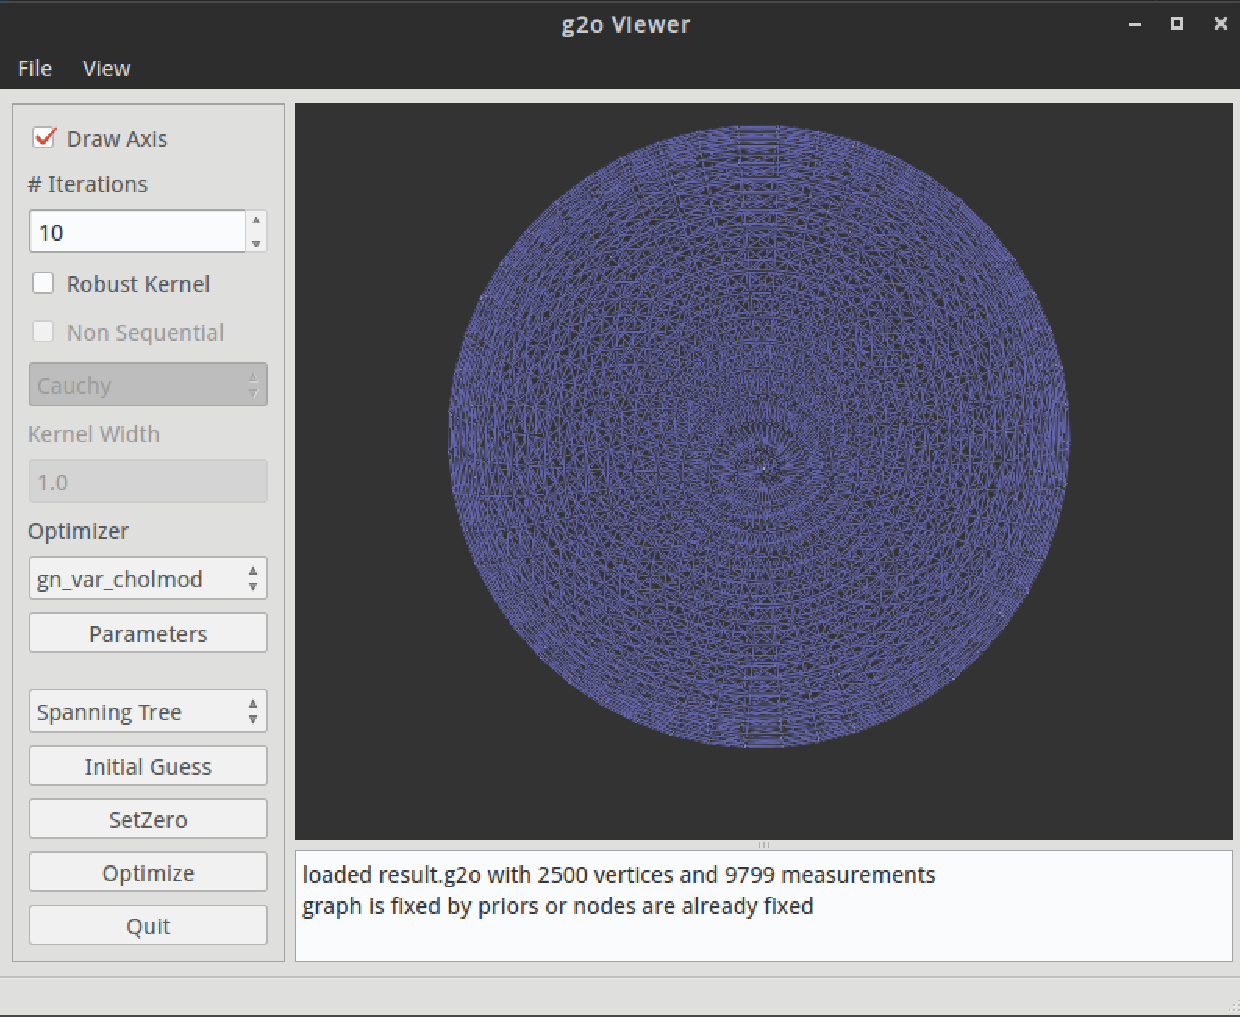
\includegraphics[width=0.75\textwidth]{backend2/result-SE3.pdf}
	\caption{使用g2o自带的顶点与边求解的结果。}
	\label{fig:result-SE3}
\end{figure}

结果从一个不规则的形状优化成了一个看起来完整的球。这个过程实质上和我们单击g2o\_viewer上的Optimize按钮没有区别。下面,我们根据前面的李代数推导来实现一下李代数上的优化。

\subsection{李代数上的位姿图优化}
还记得我们用Sophus来表达李代数的事情吗?我们来试试把Sophus用到g2o中定义自己的顶点和边吧。

\clearpage
\begin{lstlisting}[language=c++,caption=slambook2/ch10/pose\_graph\_g2o\_lie\_algebra.cpp(片段)]
typedef Matrix<double, 6, 6> Matrix6d;

// 给定误差求J_R^{-1}的近似
Matrix6d JRInv(const SE3d &e) {
    Matrix6d J;
    J.block(0, 0, 3, 3) = SO3d::hat(e.so3().log());
    J.block(0, 3, 3, 3) = SO3d::hat(e.translation());
    J.block(3, 0, 3, 3) = Matrix3d::Zero(3, 3);
    J.block(3, 3, 3, 3) = SO3d::hat(e.so3().log());
    J = J * 0.5 + Matrix6d::Identity();
    return J;
}

// 李代数顶点
typedef Matrix<double, 6, 1> Vector6d;

class VertexSE3LieAlgebra : public g2o::BaseVertex<6, SE3d> {
    public:
    EIGEN_MAKE_ALIGNED_OPERATOR_NEW
    
    virtual bool read(istream &is) override {
        double data[7];
        for (int i = 0; i < 7; i++)
        is >> data[i];
        setEstimate(SE3d(
        Quaterniond(data[6], data[3], data[4], data[5]),
        Vector3d(data[0], data[1], data[2])
        ));
    }
    
    virtual bool write(ostream &os) const override {
        os << id() << " ";
        Quaterniond q = _estimate.unit_quaternion();
        os << _estimate.translation().transpose() << " ";
        os << q.coeffs()[0] << " " << q.coeffs()[1] << " " << q.coeffs()[2] << " " << q.coeffs()[3] << endl;
        return true;
    }
    
    virtual void setToOriginImpl() override {
        _estimate = SE3d();
    }
    
    // 左乘更新
    virtual void oplusImpl(const double *update) override {
        Vector6d upd;
        upd << update[0], update[1], update[2], update[3], update[4], update[5];
        _estimate = SE3d::exp(upd) * _estimate;
    }
};

// 两个李代数节点之边
class EdgeSE3LieAlgebra : public g2o::BaseBinaryEdge<6, SE3d, VertexSE3LieAlgebra, VertexSE3LieAlgebra> {
    public:
    EIGEN_MAKE_ALIGNED_OPERATOR_NEW
    
    virtual bool read(istream &is) override {
        double data[7];
        for (int i = 0; i < 7; i++)
        is >> data[i];
        Quaterniond q(data[6], data[3], data[4], data[5]);
        q.normalize();
        setMeasurement(SE3d(q, Vector3d(data[0], data[1], data[2])));
        for (int i = 0; i < information().rows() && is.good(); i++)
        for (int j = i; j < information().cols() && is.good(); j++) {
            is >> information()(i, j);
            if (i != j)
            information()(j, i) = information()(i, j);
        }
        return true;
    }
    
    virtual bool write(ostream &os) const override {
        VertexSE3LieAlgebra *v1 = static_cast<VertexSE3LieAlgebra *> (_vertices[0]);
        VertexSE3LieAlgebra *v2 = static_cast<VertexSE3LieAlgebra *> (_vertices[1]);
        os << v1->id() << " " << v2->id() << " ";
        SE3d m = _measurement;
        Eigen::Quaterniond q = m.unit_quaternion();
        os << m.translation().transpose() << " ";
        os << q.coeffs()[0] << " " << q.coeffs()[1] << " " << q.coeffs()[2] << " " << q.coeffs()[3] << " ";
        
        // information matrix 
        for (int i = 0; i < information().rows(); i++)
        for (int j = i; j < information().cols(); j++) {
            os << information()(i, j) << " ";
        }
        os << endl;
        return true;
    }
    
    // 误差计算与书中推导一致
    virtual void computeError() override {
        SE3d v1 = (static_cast<VertexSE3LieAlgebra *> (_vertices[0]))->estimate();
        SE3d v2 = (static_cast<VertexSE3LieAlgebra *> (_vertices[1]))->estimate();
        _error = (_measurement.inverse() * v1.inverse() * v2).log();
    }
    
    // 雅可比计算
    virtual void linearizeOplus() override {
        SE3d v1 = (static_cast<VertexSE3LieAlgebra *> (_vertices[0]))->estimate();
        SE3d v2 = (static_cast<VertexSE3LieAlgebra *> (_vertices[1]))->estimate();
        Matrix6d J = JRInv(SE3d::exp(_error));
        // 尝试把J近似为I?
        _jacobianOplusXi = -J * v2.inverse().Adj();
        _jacobianOplusXj = J * v2.inverse().Adj();
    }
};
\end{lstlisting}


为了实现对g2o文件的存储和读取,本节例程实现了read和write函数,并且“伪装”成g2o内置的SE3顶点,使得g2o\_viewer能够认识并渲染它。事实上,除了内部使用Sophus的李代数表示之外,从外部看起来没有什么区别。

值得注意的是这里雅可比的计算过程。我们有若干种选择:一是不提供雅可比计算函数,让g2o自动计算数值雅可比。二是提供完整或近似的雅可比计算过程。这里我们用JRInv()函数提供近似的$\bm{\mathcal{J}}_r^{-1}$。读者可以尝试把它近似为$\bm{I}$,或者干脆注释掉oplusImpl函数,看看结果会有什么区别。

之后调用g2o进行优化问题:

\begin{lstlisting}[language=sh,caption=终端输入:]
$ build/pose_graph_g2o_lie sphere.g2o    
read total 2500 vertices, 9799 edges.
optimizing ...
iteration= 0	 chi2= 626657736.014949	 time= 0.549125	 cumTime= 0.549125	 edges= 9799	 schur= 0	 lambda= 6706.585223	 levenbergIter= 1
iteration= 1	 chi2= 233236853.521434	 time= 0.510685	 cumTime= 1.05981	 edges= 9799	 schur= 0	 lambda= 2235.528408	 levenbergIter= 1
iteration= 2	 chi2= 142629876.750105	 time= 0.557893	 cumTime= 1.6177	 edges= 9799	 schur= 0	 lambda= 745.176136	 levenbergIter= 1
iteration= 3	 chi2= 84218288.615592	 time= 0.525079	 cumTime= 2.14278	 edges= 9799	 schur= 0	 lambda= 248.392045	 levenbergIter= 1
......
\end{lstlisting}

我们发现,迭代23次后,总体误差保持不变,事实上可以让优化算法停止了。而上一个实验中,用满了30次迭代后误差仍在下降\footnote{请注意,尽管数值上看此处的误差要大一些,但是由于我们自定义边时重新定义了误差的计算方式,所以此处数值的大小并不能直接用于比较。}。在调用优化后,查看result\_lie.g2o观察它的结果,如\autoref{fig:result-lie}~所示。从肉眼上看不出任何区别。

\begin{figure}[!ht]
	\centering
	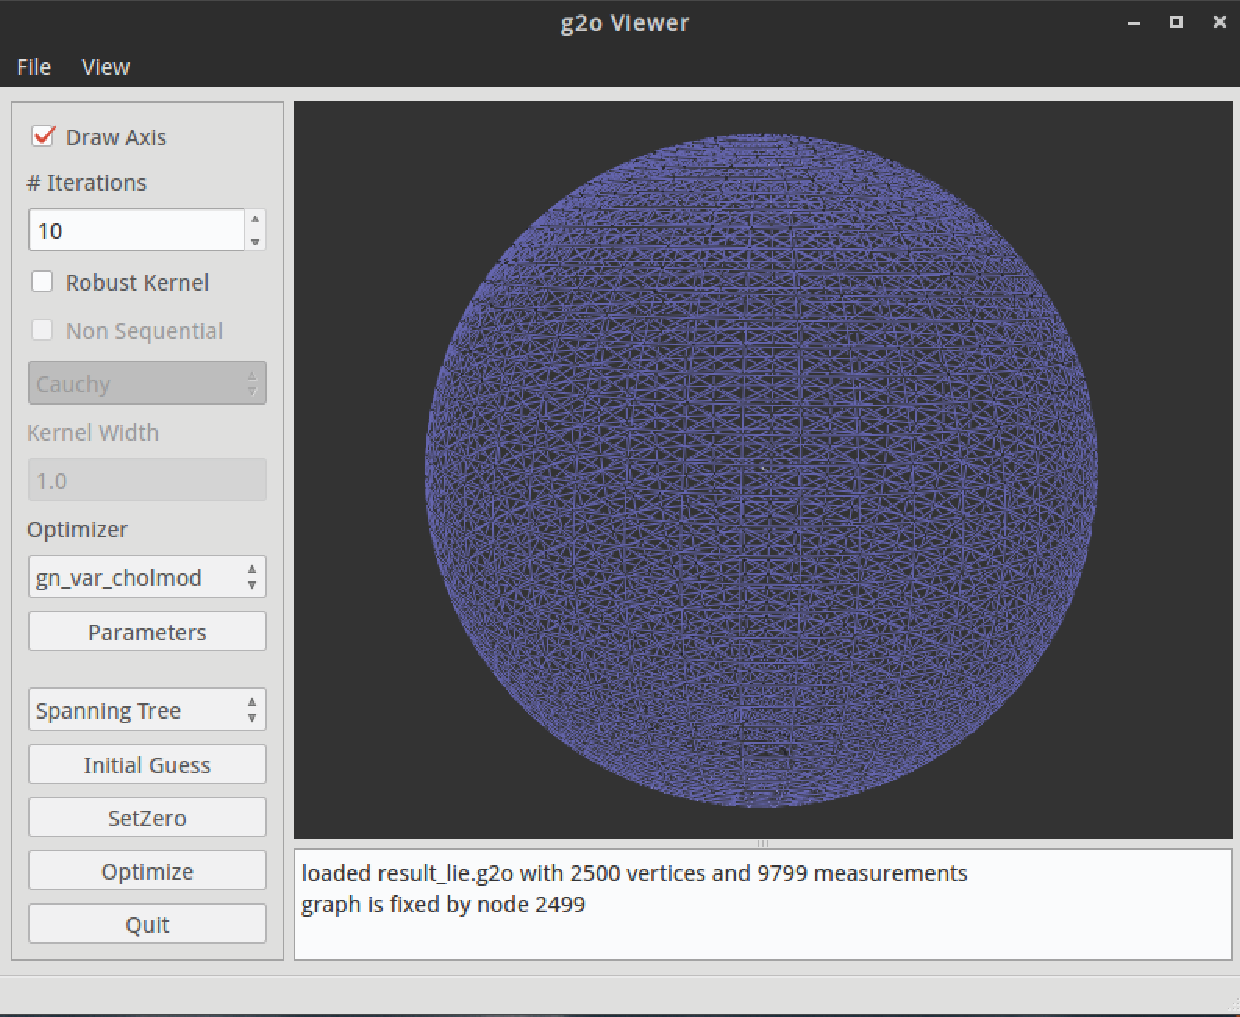
\includegraphics[width=0.72\textwidth]{backend2/result-lie.pdf}
	\caption{使用李代数自定义节点与边优化后的结果。}
	\label{fig:result-lie}
\end{figure}

如果你在这个g2o\_viewer界面按下Optimize按钮,g2o将使用它自带的SE3顶点进行优化,你可以在下方文本框中看到:

\begin{lstlisting}
loaded result_lie.g2o with 2500 vertices and 9799 measurements
graph is fixed by node 2499
# Using CHOLMOD poseDim -1 landMarkDim -1 blockordering 0
Preparing (no marginalization of Landmarks)
iteration= 0 chi2= 44360.509723 time= 0.567504 cumTime= 0.567504 edges= 9799 schur= 0
iteration= 1 chi2= 44360.471110 time= 0.595993 cumTime= 1.1635   edges= 9799 schur= 0
iteration= 2 chi2= 44360.471110 time= 0.582909 cumTime= 1.74641  edges= 9799 schur= 0
\end{lstlisting}

整体误差在SE3边的度量下为44360,略小于之前30次迭代时的44811。这说明使用李代数进行优化后,我们在更少的迭代次数下得到了更好的结果\footnote{由于没有做更多的实验,所以该结论只在“球”这个例子上有效。}。实际上,即使我们用单位矩阵来近似$\bm{\mathcal{J}}_r^{-1}$,你也会收敛到类似的值。这主要是因为在误差接近零时,雅可比本来就和恒等矩阵十分接近。

\subsection{小结}
球的例子是一个比较有代表性的案例。它具有和实际中相似的里程计边(Odometry)和回环边(Loop Closure),这也正是实际SLAM中一个位姿图中可能有的东西。同时,“球”也具有一定的计算规模:它总共有2,500个位姿节点和近10,000条边,我们发现优化它费了不少时间(相对于实时性要求很强的前端来说)。另一方面,一般认为位姿图是结构最简单的图之一。在我们不假设机器人如何运动的前提下,很难再进一步讨论它的稀疏性了——因为机器人可能会直线往前运动,形成带状的位姿图,是稀疏的;也可能是“左手右手一个慢动作”,形成大量的小型回环需要优化(Loopy motion),从而变成像“球”那样比较稠密的位姿图。无论如何,在没有进一步的信息之前,我们似乎无法再利用位姿图的求解结构了。

自PTAM\textsuperscript{\cite{Klein2007}}提出以来,人们就意识到,后端的优化没必要实时地响应前端的图像数据。人们倾向于把前端和后端分开,运行于两个独立线程之中,历史上称为跟踪(Tracking)和建图(Mapping)——虽然如此叫,建图部分主要是指后端的优化内容。通俗地说,前端需要实时响应视频的速度,例如每秒30帧;而优化可以慢悠悠地运行,只要在优化完成时把结果返回给前端即可。所以我们通常不会对后端优化提出很高的速度要求。



\section*{习题}
\begin{enumerate}
	\item 如果将位姿图中的误差定义为$\Delta \bm{\xi}_{ij} = \bm{\xi}_i \circ \bm{\xi}_j^{-1}$,推导按照此定义的左乘扰动雅可比矩阵。
    \item 如果使用右乘更新,请推导该情况下的雅可比矩阵。
	\item 参照g2o的程序,在Ceres中实现对“球”位姿图的优化。
	\item 对“球”中的信息按照时间排序,分别喂给g2o和gtsam优化,比较它们的性能差异。
	\item[\optional] 阅读iSAM相关论文,理解它是如何实现增量式优化的。
\end{enumerate}
